% Theory part of the module.
%
% Module TH-3 of Section 6.7 of the syllabus: "ML workflow and life cycle.
% The stages of an ML project from the problem definition to monitoring, and
% the feedback between the stages." Type T, 50 minutes.
%
% Sources: Volume I, chapter 3 of the textbook (the six stages, the three
% constraint layers, constraint propagation, the stage contracts, the
% fallacies) and the slide deck of the same chapter. The exercise is new: the
% syllabus gives no exercise for this module.
%
% The numbers of this module have three origins. Each frame says so in its
% source line.
% 1. A number that the textbook reports: the survey of 2016, the images
%    rejected in the clinics of Thailand, the order of magnitude of the
%    dataset. The source line names the textbook and the chapter.
% 2. The illustrative cost model of the textbook. Nobody measured it. The
%    source line says so.
% 3. A value of this course: the parameter count of MobileNetV2.
%
% Size: 15 to 25 frames for 50 minutes of theory.
%
% All diagrams are drawn again with TikZ, except for the three figures that are
% adopted from the textbook. Rule 3 of ATTRIBUTION.md gives the change of each
% redrawn diagram and the source of each adopted figure.

% ------------------------------------------------------- 1. the failed project
\begin{frame}{A project that failed at the last step}
  \begingroup\centering
  \begin{tikzpicture}[font=\scriptsize, >=stealth,
      st/.style={draw=coolgray, rounded corners=2pt, fill=boxgray,
                 align=center, text width=1.55cm, minimum height=0.95cm}]
    \node[st] (d1)  at (0,0)      {+1 day\\ build a model};
    \node[st] (d90) at (2.15,0)   {+90 days\\ 95 percent};
    \node[st] (d120) at (4.3,0)   {+120 days\\ 96 percent};
    \node[st] (d150) at (6.45,0)  {+150 days\\ hand over};
    \node[st, fill=cardinalred!12] (d152) at (8.6,0)
      {+152 days\\ the tablet has 512 MB};
    \draw[->] (d1) -- (d90); \draw[->] (d90) -- (d120);
    \draw[->] (d120) -- (d150); \draw[->] (d150) -- (d152);
  \end{tikzpicture}\par\endgroup
  \vskip 0.5em
  \small
  \begin{itemize}
    \item The model needs 4 GB of memory. The tablets of the mobile clinics
          have 512 MB. Five months of work is discarded.
    \item The accuracy was good. The skills of the team were good. The
          failure was a workflow failure.
  \end{itemize}
\end{frame}

% --------------------------------------------------------- 2. what a lifecycle is
\begin{frame}{What the machine learning lifecycle is}
  \begin{itemize}
    \item A structure for the work, not a method for one model. It names
          the stages of a project and the output of each stage.
    \item It is iterative. A stage sends its result back to an earlier
          stage as often as it needs to.
    \item It covers the running system. Monitoring is a stage of the
          project, not the end of it.
  \end{itemize}
  \vskip 0.4em
  \keypoint{The lifecycle is a loop, not a list.}
\end{frame}

% ------------------------------------------------------------- 3. the six stages
\begin{frame}{The six stages}
  \begingroup\centering
  \begin{tikzpicture}[font=\scriptsize, >=stealth,
      st/.style={draw=coolgray, rounded corners=2pt, fill=boxgray,
                 align=center, text width=2.3cm, minimum height=0.8cm},
      lab/.style={font=\scriptsize\sffamily\bfseries, text=white,
                  fill=coolgray, rounded corners=1pt, inner sep=2pt}]
    \node[st] (a) at (0,0)    {Problem\\ definition};
    \node[st] (b) at (2.75,0)  {Data collection\\ and preparation};
    \node[st] (c) at (5.5,0)  {Model\\ development};
    \node[st] (d) at (2.75,-1.9) {Evaluation\\ and validation};
    \node[st] (e) at (0,-1.9)  {Deployment\\ and integration};
    \node[st] (f) at (-2.75,-1.9) {Monitoring\\ and maintenance};
    \draw[->] (a) -- (b); \draw[->] (b) -- (c);
    \draw[->] (c.south) |- (d.east);
    \draw[->] (d) -- (e); \draw[->] (e) -- (f);
    \draw[cardinalred, dashed] (f.north) -- (-2.75,0.95);
    \draw[->, cardinalred, dashed] (-2.75,0.95) --
      node[above, font=\scriptsize] {feedback} (2.75,0.95) -- (b.north);
  \end{tikzpicture}\par\endgroup
  \vskip 0.9em
  \small
\end{frame}

% ------------------------------------------------- 3b. the named feedback paths
\begin{frame}{Every feedback path has a name}
  \begingroup\centering
  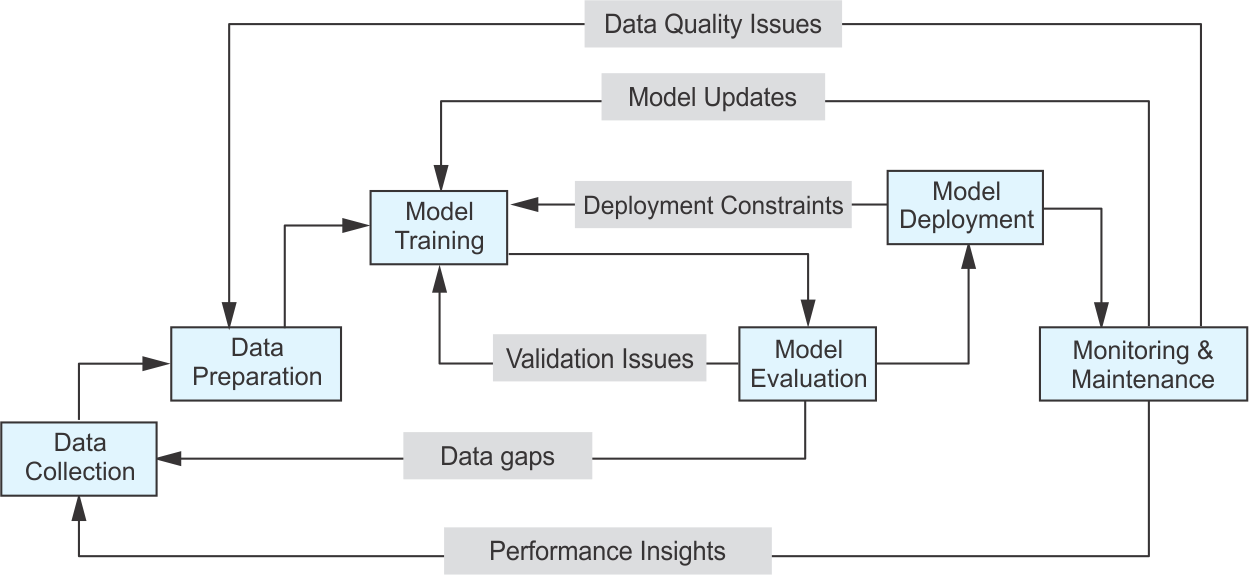
\includegraphics[width=\textwidth]{images/modules/TH-3/feedback_loops.png}
  \par\endgroup
  \vskip 0.3em
  \small
  The grey boxes name what travels back. Data gaps send the team to the
  collection. Deployment constraints go back to the training. Performance
  insights from the running system decide what happens next.
  \source{Figure adopted from Volume I, chapter 3.}
\end{frame}

% ------------------------------------------------------------- 4. the stage table
\begin{frame}{The output of each stage}
  \footnotesize
  \begin{tabular}{@{}L{2.5cm}L{6.6cm}@{}}
    \toprule
    Stage & Output that the next stage needs \\
    \midrule
    Problem definition & Targets, the deployment device, the budgets \\
    Data collection & A versioned dataset, the preparation code \\
    Model development & Weights, the training configuration \\
    Evaluation & Metrics per subgroup, the list of failure modes \\
    Deployment & The running system, the instruments, the rollback \\
    Monitoring & The alerts, the review, the incident reports \\
    \bottomrule
  \end{tabular}
  \vskip 0.5em
  \small Each stage is complete when its output exists and passes its check.
  A stage that ends without a check gives the next stage a defect.
\end{frame}

% ------------------------------------------------------------ 5. where time goes
\begin{frame}{Where the engineering time goes}
  \begingroup\centering
  \begin{tikzpicture}[font=\scriptsize, x=0.11cm, y=0.42cm, >=stealth]
    \node[anchor=east] at (-0.15,0) {Cleaning data};
    \fill[treegreen!55] (0,-0.28) rectangle (60,0.28);
    \node[anchor=west] at (60,0) {60 percent};
    \node[anchor=east] at (-0.15,1) {Collecting data};
    \fill[treegreen!55] (0,0.72) rectangle (19,1.28);
    \node[anchor=west] at (19,1) {19 percent};
    \node[anchor=east] at (-0.15,2) {Mining patterns};
    \fill[treegreen!55] (0,1.72) rectangle (9,2.28);
    \node[anchor=west] at (9,2) {9 percent};
    \node[anchor=east] at (-0.15,3) {Building training sets};
    \fill[treegreen!55] (0,2.72) rectangle (3,3.28);
    \node[anchor=west] at (3,3) {3 percent};
    \node[anchor=east] at (-0.15,4) {Refining algorithms};
    \fill[treegreen!55] (0,3.72) rectangle (4,4.28);
    \node[anchor=west] at (4,4) {4 percent};
    \node[anchor=east] at (-0.15,5) {Other};
    \fill[treegreen!55] (0,4.72) rectangle (5,5.28);
    \node[anchor=west] at (5,5) {5 percent};
    \end{tikzpicture}\par\endgroup
  \vskip 0.5em
  \small
  \begin{itemize}
    \item 79 percent of the reported time goes to collecting and cleaning
          data. 16 percent goes to model work.
    \item Data engineering is not preparation. It is most of the project.
  \end{itemize}
  \source{CrowdFlower, \emph{Data Science Report 2016}, as reported in
    Volume I, chapter 3.}
\end{frame}

% --------------------------------------------------------- 6. not software
\begin{frame}{ML is not software with a model}
  \footnotesize
  \begin{tabular}{@{}L{3.1cm}L{3.1cm}L{3.1cm}@{}}
    \toprule
    & Written software & A learned system \\
    \midrule
    Specification & Exact functions & A statistical behaviour \\
    Test & One expected result & A distribution with uncertainty \\
    Deployment & Static until an update & Changes when the data changes \\
    Maintenance & Fix the code & Watch the data, then retrain \\
    \bottomrule
  \end{tabular}
  \vskip 0.5em
  \small The behaviour of a learned system comes from the training data.
  Changing the data changes the behaviour with no change in the code.
\end{frame}

% --------------------------------------------------- 7. problem definition
\begin{frame}{Stage 1: what a problem definition states}
  \small
  \begin{itemize}
    \item The behaviour to reach, as a number that a test can check. An
          average accuracy hides a subgroup that fails.
    \item The device and its budgets: memory, latency, power, and the
          network.
    \item The operating rules: privacy, audit, and who accepts the result.
  \end{itemize}
  \vskip 0.4em
  \keypoint{Write the constraint before the architecture.}
\end{frame}

% --------------------------------------------------- 8. constraint layers
\begin{frame}{The three layers of constraints}
  \begingroup\centering
  \begin{tikzpicture}[font=\scriptsize, >=stealth,
      st/.style={draw=coolgray, rounded corners=2pt, fill=boxgray,
                 align=center, text width=2.7cm, minimum height=1.5cm}]
    \node[st] (s) at (0,0) {Statistical\\ sensitivity, accuracy\\ per subgroup};
    \node[st] (p) at (3.2,0) {Physical\\ memory, latency,\\ power, thermal};
    \node[st] (o) at (6.4,0) {Operational\\ privacy, audit,\\ who accepts it};
    \draw[->, cardinalred] (s) -- node[above, font=\scriptsize] {limits} (p);
    \draw[->, cardinalred] (p) -- node[above, font=\scriptsize] {limits} (o);
  \end{tikzpicture}\par\endgroup
  \vskip 0.5em
  \small A constraint in one layer removes options in the other two. A model
  that is too large for the device pushes the work back to the architecture,
  and a missing audit rule can force a retraining later.
\end{frame}

% --------------------------------------------------- 9. propagation
\begin{frame}{Constraints propagate backward}
  \begingroup\centering
  \begin{tikzpicture}[font=\scriptsize, >=stealth,
      st/.style={draw=coolgray, rounded corners=2pt, fill=boxgray,
                 align=center, text width=1.4cm, minimum height=0.7cm}]
    \node[st] (s1) at (0,0)    {1 target};
    \node[st] (s3) at (2.8,0)   {3 model};
    \node[st] (s5) at (5.6,0)   {5 deploy};
    \node[st, fill=cardinalred!12] (s6) at (8.4,0) {6 monitoring};
    \draw[->] (s1) -- (s3); \draw[->] (s3) -- (s5); \draw[->] (s5) -- (s6);
    \draw[->, cardinalred, dashed] (s6.south) -- ++(0,-0.85)
      -| node[pos=0.5, below, font=\scriptsize, text=cardinalred,
        text width=3.0cm, align=center]
      {the memory limit was known on the first day} (s1.south);
  \end{tikzpicture}\par\endgroup
  \vskip 0.5em
  \small
  A limit that nobody writes in the problem definition does not disappear.
  It comes back at the stage that meets it, and it invalidates every
  decision that was made after the day it should have been known.
  \source{Principle of Volume I, chapter 3.}
\end{frame}

% --------------------------------------------------- 10. the cost model
\begin{frame}{A cost model for a late constraint}
  \begin{equation*}
    \text{correction cost} \approx 2^{\,N-1} \times \text{stage 1 cost}
  \end{equation*}
  \small
  \begin{center}
  \footnotesize
  \begin{tabular}{@{}lrrrrr@{}}
    \toprule
    Found at stage & 2 & 3 & 4 & 5 & 6 \\
    \midrule
    Multiple of the stage 1 cost & 2 & 4 & 8 & 16 & 32 \\
    \bottomrule
  \end{tabular}
  \end{center}
  \vskip 0.3em
  \small This model is an illustration, not a measured law. It shows the
  shape of the effect: each earlier stage that the correction passes through
  adds its own validation and testing work.
  \source{Illustrative model of Volume I, chapter 3, after Boehm (1981).}
\end{frame}

% ------------------------------------------------ 10b. the cost curve
\begin{frame}{The cost curve of a late constraint}
  \begingroup\centering
  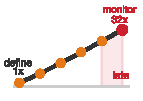
\includegraphics[width=0.72\textwidth]{images/modules/TH-3/ml_workflow_constraint_cost_escalation.pdf}
  \par\endgroup
  \vskip 0.4em
  \small
  The curve is not straight. Each stage that the correction passes through
  adds its own validation and testing, so the curve steepens. A limit found
  at monitoring costs 32 times the same limit found at the problem
  definition.
  \source{Figure adopted from Volume I, chapter 3.}
\end{frame}

% --------------------------------------------------- 11. data collection
\begin{frame}{Stage 2: data collection and preparation}
  \small
  \begin{itemize}
    \item The targets of stage 1 become data requirements. A model that
          must run on the kit needs inputs that the kit produces.
    \item The dataset has a version. Without it no earlier result can be
          reproduced.
    \item Preparation is code, so it changes, so it needs a test.
  \end{itemize}
  \vskip 0.4em
  \small A screening system of this kind needs images on the order of
  $10^5$, each read by several specialists, because one reader disagrees
  with another on the border cases.
  \source{Order of magnitude of Volume I, chapter 3.}
\end{frame}

% --------------------------------------------------- 12. the lab to field gap
\begin{frame}{The lab-to-field data gap}
  \begin{itemize}
    \item A screening model reached the accuracy of a specialist in the
          laboratory.
    \item In the clinics of Thailand, 393 of 1 838 submitted images (21
          percent) failed the image quality check of the system.
    \item The cause was the room, the camera, and the practice of the
          clinic. No change in the model would have helped.
  \end{itemize}
  \vskip 0.4em
  \keypoint{A dataset that matches the laboratory does not match the site.}
  \source{Beede and others (2020), as reported in Volume I, chapter 3.}
\end{frame}

% --------------------------------------------------- 13. model development
\begin{frame}{Stage 3: model development}
  \small
  \begin{itemize}
    \item The architecture is chosen inside the budget of stage 1, not
          after it.
    \item MobileNetV2 has 3 504 872 parameters. In \code{float32} the
          weights alone need 13.4 MB. A tablet with 512 MB can hold the
          model, but the input pipeline and the runtime still need room.
    \item The training configuration is an output of this stage. Without it
          the weights cannot be rebuilt.
  \end{itemize}
\end{frame}

% --------------------------------------------------- 14. evaluation
\begin{frame}{Stage 4: evaluation and validation}
  \small
  \begin{itemize}
    \item One number is not enough. Report the metric per subgroup that
          the problem definition named.
    \item Fix the threshold here. The threshold is part of the system, so
          it needs a test.
    \item Test on data that no stage has touched, and keep it that way.
    \item Test on the device. A model that passes on a laptop can fail on
          the target with a different number format.
  \end{itemize}
\end{frame}

% --------------------------------------------------- 15. deployment
\begin{frame}{Stage 5: deployment and integration}
  \small
  \begin{itemize}
    \item The model is now one part of a running system. The path from the
          sensor to the result decides the latency.
    \item Write down what the system promises: latency, uptime, and the
          behaviour when a stage fails.
    \item Keep a way back. A version that fails in the field must be
          replaceable by the version before it.
    \item Check the whole path on the device. A model that runs alone is
          not a system.
  \end{itemize}
\end{frame}

% --------------------------------------------------- 16. monitoring
\begin{frame}{Stage 6: monitoring and maintenance}
  \begingroup\centering
  \begin{tikzpicture}[font=\scriptsize, >=stealth, x=1cm, y=1cm]
    \draw[thick, cardinalred] (0,2.30) -- (3.6,2.30)
      -- (4.4,2.05) -- (5.2,1.75) -- (6.0,1.45)
      -- (7.0,1.20) -- (8.0,1.05) -- (9.2,0.98);
    \draw[thick, coolgray, line width=1.4pt] (0,2.30) -- (9.2,2.30);
    \node[anchor=south east, text=coolgray] at (9.2,2.42)
      {the accuracy the model was validated at};
    \node[anchor=north east, text=cardinalred] at (9.2,0.90)
      {the accuracy at the clinic};
    \draw[dashed, coolgray] (3.6,0) -- (3.6,3.05);
    \node[anchor=south, text=coolgray] at (3.6,3.10)
      {the clinic buys new cameras};
    \draw[<->, cardinalred] (6.9,1.32) -- (6.9,2.30);
    \node[anchor=west, text=cardinalred] at (7.0,1.80) {the gap};
    \draw[->] (0,0) -- (9.7,0) node[right, font=\scriptsize] {time};
  \end{tikzpicture}\par\endgroup
  \vskip 0.5em
  \begingroup\centering
  \begin{tikzpicture}[font=\scriptsize, >=stealth,
      bx/.style={draw=coolgray, rounded corners=2pt, fill=boxgray,
                 align=center, text width=2.5cm, minimum height=0.75cm}]
    \node[bx] (m) at (0,0)    {the monitoring sees the gap};
    \node[bx] (r) at (3.1,0)  {a review starts};
    \node[bx] (d) at (6.2,0)  {the team decides what to change};
    \draw[->] (m) -- (r);
    \draw[->] (r) -- (d);
  \end{tikzpicture}\par\endgroup
  \vskip 0.4em
  \small No line of code changed, so nothing failed and no error was
  raised. The gap between the two lines is the whole reason that stage 6
  is a stage of the project.
\end{frame}

% --------------------------------------------------- 17. feedback speeds
\begin{frame}{Feedback runs at three speeds}
  \footnotesize
  \begin{tabular}{@{}L{3.0cm}L{2.6cm}L{4.2cm}@{}}
    \toprule
    Review & Period & Finds \\
    \midrule
    Live monitoring & Seconds & A stopped service, a sensor that fails \\
    Update review & Days & Drift, a fall in a metric, a new subgroup \\
    Architecture review & Months & A budget that no longer holds \\
    \bottomrule
  \end{tabular}
  \vskip 0.5em
  \small One loop for all three does not work. A fast loop that waits for
  the slow reviews reacts too late. A slow loop that runs on every alert
  spends its budget with no signal.
\end{frame}

% ------------------------------------------------ 17b. the timescale ladder
\begin{frame}{The span of the review periods}
  \begin{columns}[T]
    \begin{column}{0.34\textwidth}
      \centering
      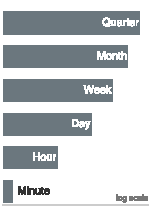
\includegraphics[height=4.6cm]{images/modules/TH-3/ml_workflow_feedback_timescales.pdf}
    \end{column}
    \begin{column}{0.62\textwidth}
      \small
      \begin{itemize}
        \item The periods of a real system span five orders of magnitude,
              from a minute to a quarter.
        \item The diagram uses a logarithmic scale. Each bar is one period.
        \item A drift signal needs a day loop. A change of the budget needs
              a quarter loop.
      \end{itemize}
    \end{column}
  \end{columns}
  \source{Figure adopted from Volume I, chapter 3.}
\end{frame}

% --------------------------------------------------- 18. contracts
\begin{frame}{Stage contracts}
  \small Every stage has an input, an output, and a condition that the
  output must satisfy. The team checks the condition at the door of the next
  stage, while the fix is still one change.
  \vskip 0.3em
  \footnotesize
  \begin{tabular}{@{}L{4.1cm}L{5.3cm}@{}}
    \toprule
    Contract & Example of a condition \\
    \midrule
    Problem definition & Every target has a number \\
    Data collection & The data matches the site \\
    Model development & The model fits the budget \\
    Evaluation & No named subgroup is below its floor \\
    Deployment & The latency and the uptime hold \\
    Monitoring & An alert starts a review \\
    \bottomrule
  \end{tabular}
\end{frame}

% --------------------------------------------------- 19. fallacies
\begin{frame}{Three fallacies}
  \small
  \begin{itemize}
    \item \textbf{An ML project can follow a software plan.} The targets
          move when the data shows a gap, so the plan moves with them.
    \item \textbf{Data preparation is a step that ends.} The data of the
          site changes after the launch, so preparation is a running
          pipeline.
    \item \textbf{A good model means a good system.} The number of the
          model says nothing about the latency, the recovery, or the cost
          of the device.
  \end{itemize}
  \vskip 0.4em
  \keypoint{Optimising one stage moves the failure. It does not remove it.}
\end{frame}

% --------------------------------------------------- 20. summary
\begin{frame}{What to remember}
  \small
  \begin{enumerate}
    \item Six stages, and an output that the next stage checks.
    \item Three layers of constraints: statistical, physical, operational.
    \item A constraint that nobody writes down returns later, and it
          returns as a redesign.
    \item Monitoring is a stage of the project. It sends work back to the
          data and to the model.
    \item Every feedback loop has its own speed and its own review.
  \end{enumerate}
\end{frame}

% --------------------------------------------------- exercise
\exerciseframe{Late constraint}{A team finds during monitoring (stage 6)
that its model fails for the images of one clinic. The limit of that clinic
was never written in the problem definition.

\begin{enumerate}
  \item Give the cost multiplier of the illustrative model.
  \item Name the stages that the team must revisit.
\end{enumerate}

Work in pairs for 5 minutes.}

\answerframe{Late constraint}{
  \begin{enumerate}
    \item The constraint is found at stage 6, so the multiplier is
          $2^{6-1} = 32$ times the cost of the same correction at stage 1.
    \item Stages 2 to 5: more data for that clinic, a new model, a new
          evaluation, and a new version on the devices.
  \end{enumerate}
  \vskip 0.3em
  \small The 32 is an illustration, not a measurement. The part that
  carries over to real work is the list of stages: the correction of a late
  constraint passes through every stage between.}